\documentclass{article}
% Choose a conveniently small page size
% PACKAGES
\usepackage[margin = 1in]{geometry}
\usepackage{amsfonts}
\usepackage{amsmath}
\usepackage{amssymb}
\usepackage{multicol}
\usepackage{graphicx}
\usepackage{float}
\usepackage{xcolor}
\usepackage{amsthm}
\usepackage{dsfont}
\usepackage{hyperref}

% MACROS
% Set Theory
\def\N{\mathbb{N}}
\def\R{\mathbb{R}}
\def\C{\mathbb{C}}
\def\Z{\mathbb{Z}}
%\def\^{\hat}
\def\-{\vec}
\def\d{\partial}
\def\!{\boldsymbol}
\def\X{\times}
%\def\-{\bar}
\def\bf{\textbf}
\def\l{\left}
\def\r{\right}
\title{Summer Internship for Damien Beecroft}
\author{Advisors: Amanda Howard, Panos Stinis}
\begin{document}
\maketitle
Physics-informed neural networks, or PINNs, have shown great promise in learning the solution to partial differential equations. However, there are still cases where PINNs fail to train. This summer, we will develop new techniques for cases where PINNs fail to train.
\par This document serves only as a suggested outline, and creativity is encouraged. The remaining weeks will be filled in as we see how the results develop. Many extensions are possible, including training deep operator networks (DeepONets) for a range of input parameters, or switching to model other dynamical systems. 
\par The suggested reading for each week consists of background information that you may find helpful as you work. I suggest you write a short, 1-2 sentence, summary of each paper and add it a working document after reading each paper. This will be the introduction to your final report, and later the introduction for a publication based on your work. Articles are available through PNNL when you’re logged into the VPN.
\begin{figure}[H]
\center
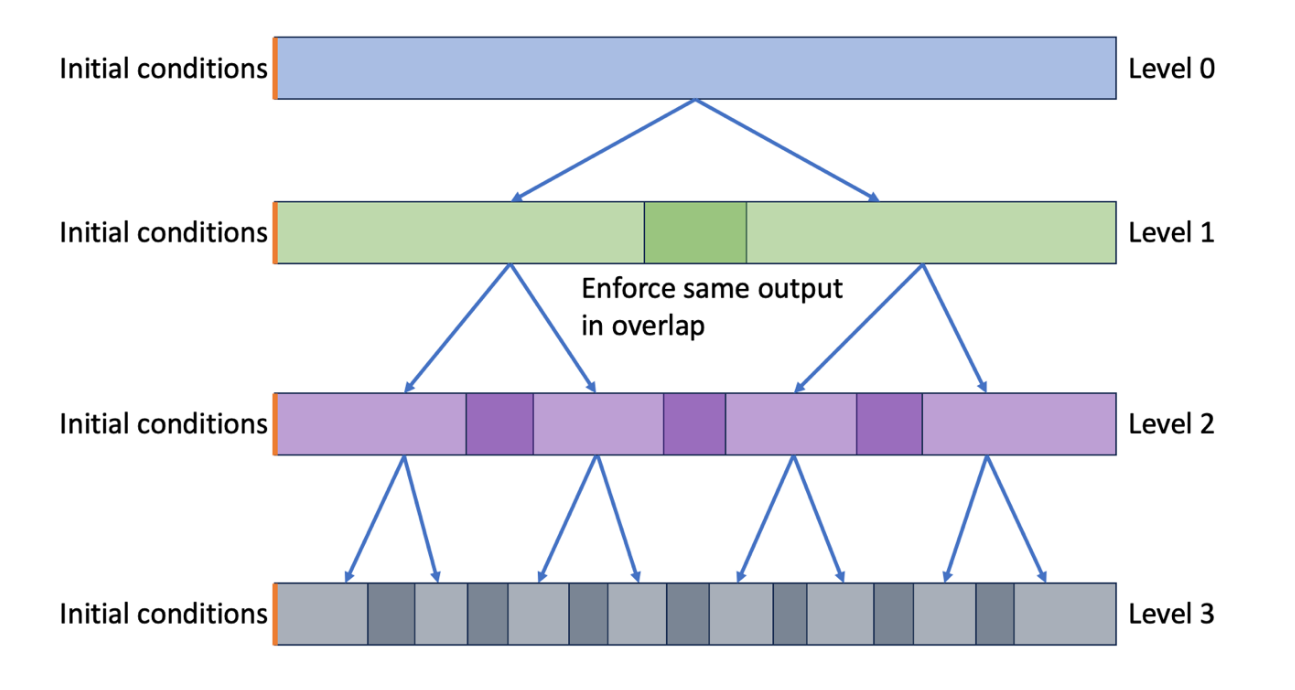
\includegraphics[width=0.8\textwidth]{imgs/domain_decomp}
\end{figure}
We will consider a multifidelity domain decomposition approach, where a PINN is trained in the full domain first. Then, the full domain training is used as a low fidelity prediction for a prediction in a subdivided domain. Two PINNs are trained in level 1, and the domains overlap so initial conditions are not needed to train the subdomain that occurs for later time. This process is repeated until the desired accuracy is reached across the domain.  
\par We will be working with Alexander Heinlein, who is an expert in domain decomposition. We will start by testing this setup on the case of an undamped pendulum, to see if we can overcome the issue of converging to fixed points for long time. If successful, we will move to more complex examples. Creativity is encouraged in designing training algorithms. 
\newpage
\subsection*{To Do}
\bf{Reading}:
\begin{itemize}
	\item Parallel Physics-Informed Neural Networks via Domain Decomposition: \url{https://arxiv.org/pdf/2104.10013.pdf}
	\item Fourier Analysis Sheds Light on Deep Neural Networks: \url{https://arxiv.org/abs/1901.06523}
\end{itemize}
\bf{Coding}:
\begin{itemize}
	\item Do Now
	\begin{itemize}
		\item You can precompute the weights that correspond to each batch ahead of time and generate them in the batch.
		\item Preselect the points in the batch. Don't randomly choose some points in each batch.
		\item Make the batching more efficient. Generate the weights for the newest level inside of the batch.
		\item Given a time scale that trains, decrease the network size until failure.
		\item Work on implementing the wave equation
		\item Make the multifidelity code efficient
	\end{itemize}
	\item Pendulum
	\begin{itemize}
		\item Run the domain decomposition code in \verb|Pendulum_DD|
		\item Point selection and evaluation
		\begin{itemize}
			\item Make sure that the code does not evaluate every network at all points. Only evaluate networks on points within the support of their weight function. There are two potential methods for how to do this.
			\begin{itemize}
				\item Change the data generator function to only generate output points in a given domain 
				\item Once you are given a point, check whether or not the point is in the support of the weight function.
			\end{itemize}
			\item Work on parallelization of neural networks defined on different sub-domains.
			\item Testing
			\begin{itemize}
				\item Running with and without the residual driven point selection
				\item Look at the sensitivity of the weights of the loss function
			\end{itemize}
			\item Do testing on how high we can get the maximum time of the pendulum. Currently it is at 10. Can we get it to 20? 50?
		\end{itemize}
	\end{itemize}


	\item Wave Equation
%	\begin{itemize}
%		\item 
%	\end{itemize}
	\item Allen-Cahn
%	\begin{itemize}
%		\item 
%	\end{itemize}
	\item Lorenz
%	\begin{itemize}
%		\item 
%	\end{itemize}
\end{itemize}

\newpage
\newpage
\subsection*{Week 1}
\bf{Videos}:
\begin{itemize}
	\item Stanford CS229M Lecture 13 (Neural Tangent Kernel): \url{https://www.youtube.com/watch?v=btphvvnad0A&list=RDCMUCBa5G_ESCn8Yd4vw5U-gIcg&index=1}
\end{itemize}
\bf{Reading}:
\begin{itemize}
	\item PINNs: \url{https://www.sciencedirect.com/science/article/pii/S0021999118307125}
	\item Multifidelity PINN: \url{https://arxiv.org/pdf/1903.00104.pdf}
	\item Multifidelity DeepONets: \url{https://arxiv.org/pdf/2204.09157.pdf}
	\item Multifidelity Continual Learning: \url{https://arxiv.org/pdf/2304.03894.pdf}
	\item Fixed points and PINNs: \url{https://arxiv.org/pdf/2203.13648.pdf}
	\item Multilevel Domain Decomposition for PINNs: \url{https://arxiv.org/pdf/2306.05486.pdf}
	\item Point selection for PINNs: \url{https://www.sciencedirect.com/science/article/pii/S0045782522006260}
	\item Respecting Causality is All you Need: \url{https://arxiv.org/pdf/2203.07404.pdf}
\end{itemize}
\bf{Coding}:\\
\par I was sent the pendulum code by Amanda. I took some time this week to go through it and get a feel for what is going on. I have not run the code since I do not have my PNNL laptop. I plan to have the code up and running early next week.
%\newpage
\subsection*{Week 2}
\bf{Reading}:
\begin{itemize}
	\item A Method for Representing Periodic Functions and Enforcing Exactly Periodic Boundary Conditions with Deep Neural Networks: \url{https://arxiv.org/pdf/2007.07442.pdf}
	\item How and Why PINNs Fail to Train: \url{https://arxiv.org/pdf/2007.14527.pdf}
	\begin{itemize}
		\item Neural Tangent Kernel Convergence and Generalization: \url{https://arxiv.org/abs/1806.07572}
		\item Deep Neural Networks as Gaussian Processes: \url{https://arxiv.org/abs/1711.00165}
	\end{itemize}
\end{itemize}
\bf{Coding}:
\begin{itemize}
\item Get access to Marianas
\item Set up GitHub repository
\item Set up GitHub repository on Marianas and pull code from \verb|pnnl_research|
\item Run Amanda's code locally
\item Plot solutions from Amanda's code
\item Tried to get \verb|onet_scripts| running on Marianas. It did not work.
\end{itemize}
%\newpage
\subsection*{Week 3} 
\bf{Notes}:
\begin{itemize}
\item Tried to get \verb|onet_scripts| running on Marianas. It did not work. I spent a lot of time on this.
\item I went through the original code Amanda sent me slowly to understand exactly how it works.
\item I went through the altered code in \verb|Pendulum_DD| to understand exactly how it works. This was rather time consuming.
\item I realized that the problem of only applying neural networks to points within their domains can be solved with a rather simple sorting algorithm.
\end{itemize}
\subsection*{Coding}
\begin{itemize}
\item Implementing domain sorting code.
\end{itemize}

%\newpage
\subsection*{Week 4}
\bf{Coding}
\begin{itemize}
\item I created a function that sorts the points amongst the tree of domains.
\item I created a super class that tracks which nodes are on which levels of the tree.
\item I created a function that evaluates the nodes on each level and sorts them accordingly.
\item I began taking the code apart and putting it back together in order to get things working.
\end{itemize}
%\newpage
\subsection*{Week 5} 
\bf{Coding}
\begin{itemize}
\item This week I went to the PNNL office in Seattle to meet  Amanda and Sarah.
\item Sarah and I met with Shady. Shady was able to figure out why Sarah and I could not get the code running on Marianas. There were extra packages in our \verb|python| and \verb|.conda| files. After deleting these packages the code ran.
\item I spent time trying to figure out how to set up the visit to Pasco. Of course, Concur got the better of me in the end and I did not end up going to Pasco.
\item I worked on integrating the theory I had worked out in week 4 in with the \verb|Pendulum_DD| code.
\item I began to have difficulties with Jax as I was beginning to integrate the code in with Amanda's.
\item I read through the Jax documentation in order understand how to implement the multifidelity network architecture.
\end{itemize}
%\newpage
\subsection*{Week 6}
\textbf{Coding}
\begin{itemize}
\item I learned about pytrees in Jax. I began attempting to translate the code that I have to be compatible with Jax.
\item I began to realize that I could not get pytrees working with in Jax, at least the way I was implementing it.
\item I talked to Amanda and she suggested that I try making batches for each subset where different neural networks are defined.
\item I tried implementing the multiple batching, however, the code was not running. Jax was again giving me problems.
\item I tried running the original \verb|Pendulum_DD| code that Amanda sent me and it gave me an error. I tried extracting the original zip file that Amanda gave me and that also gave me the same error. I cannot get the \verb|Pendulum_DD| code to run at all now. I am doubting if I ever actually ran it.
\end{itemize}
%\newpage
\subsection*{Week 7}
\textbf{Coding}
\begin{itemize}
\item I realized that \verb|Pendulum_DD| code that I was sent never ran  in the first place. It had a bug where \verb|self.NDomains| was converted to a traced value implicitly. The code then attempted to make a numpy array with this code, but this can't be done with a traced variable.
\item I did the pendulum code up to time 20. It failed to train.
\item I increased the amount of resources used on the single fidelity network for the T = [0,20] training session. The single fidelity network was a bit better, but still struggled.
\item I modified the code so that neural networks are only evaluated on points that lie within their support. However, the implementation was sloppy and the code is far slower than the code where all neural nets are evaluated everywhere.
\item I began thinking about how to make the code more efficient. I believe that the main reason is the for loops in my code and the poor batching method. I am working on changing both of these.
\end{itemize}
\newpage 
\subsection*{Week 8} 
\newpage
\subsection*{Week 9}
\newpage
\subsection*{Week 10}  
\newpage
\end{document}